%
% Auteur initial inconnu.
% Modifié par olivier.ploton@univ-tours.fr le 21/09/2021
% À compiler avec pdflatex, bibilographie avec biber.
% Tous les fichiers doivent être encodés en UTF-8
% S'utilise en présence du fichier de bibiographie biblio.bib
% et des dossiers polytech/ (classe) et pic/ (images)
%

\documentclass{polytech/polytech}
\usepackage[strings]{underscore} % utile pour les _ dans la biblio (DOI)

% Fixe la présentation des listings
\lstset{
 columns=fixed,       
 numbers=left,                              
 numberstyle=\tiny\color{gray},             
 frame=single,                              
 backgroundcolor=\color[RGB]{255,255,255},  
 keywordstyle=\color[RGB]{40,40,255},       
 numberstyle=\footnotesize\color{darkgray}, 
 commentstyle=\it\color[RGB]{0,96,96},      
 stringstyle=\rmfamily\slshape\color[RGB]{128,0,0},  
 showstringspaces=false,                    
 language=C++
}

% Quelques formatages supplémentaires
\numberwithin{figure}{chapter}
\renewcommand\thesubsection{\thesection.\arabic{subsection}} 

% dossier des images
\graphicspath{{./pic/}}

%%%%%%%%%%%%%%%%%%%%%%%%%%%%%%%%%%%%%%%%

%
% Paramètres à fixer avant de commencer le document
%

\typereport{prddi5}       

\reportyear{2021-2022}

\title{Titre du PRD}
\subtitle{sous-titre du PRD}
\reportlogo{polytech/polytech}
           
\student[di5]{Prénom}{NOM}{email@univ-tours.fr}

\academicsupervisor[di]{Prénom}{NOM}{email@univ-tours.fr}

\industrialsupervisor{Prénom}{NOM}{email@univ-tours.fr}

\company[polytech/polytech]{Polytech}
    {64 avenue Jean Portalis\\37200 Tours, France}
    {polytech.univ-tours.fr}


\resume{%
Voici le résumé de ce PRD.
Voici le résumé de ce PRD.
Voici le résumé de ce PRD.
Voici le résumé de ce PRD.
Voici le résumé de ce PRD.
Voici le résumé de ce PRD.
Voici le résumé de ce PRD.
Voici le résumé de ce PRD.
Voici le résumé de ce PRD.
}

\motcle{motcle1}
\motcle{motcle2}
\motcle{etc.}

             
\abstract{
Here is the abstract of this project.
Here is the abstract of this project.
Here is the abstract of this project.
Here is the abstract of this project.
Here is the abstract of this project.
Here is the abstract of this project.
Here is the abstract of this project.
Here is the abstract of this project.
Here is the abstract of this project.
}
\keyword{word1}
\keyword{word2}
\keyword{etc.}

%
% Le poster. Il faut exactement 3 blocs.
%

\posterblock{Objectifs}{
\begin{itemize}
\item point 1
\item point 2 
\item point 3
\end{itemize}
}{pic/lifat.png}{}

\posterblock{Mise en œuvre}{
\begin{enumerate}
\item point 1
\item point 2 
\item point 3
\end{enumerate}
}{pic/lifat.png}{}

\posterblock{Résultats attendus}{
Voici du texte.
Voici du texte.
Voici du texte.
Voici du texte.
Voici du texte.
Voici du texte.
}{pic/lifat.png}{}


\newglossaryentry{framework}
{
	name=Framework,
	description={Ensemble d'outils et de composants logiciels organisés conformément à un plan d'architecture et des patterns}
}

\newglossaryentry{opensource}
{
	name=Open Source,
	description={Libre de droits, dont les codes sources sont disponibles et modifiables librement}
}


\newacronym{uml}{UML}{Unified Modeling Language}
\newacronym{cudnn}{cuDNN}{NVIDIA CUDA Deep Neural Network}

\bibliography{biblio}
\makeglossaries

%%%%%%%%%%%%%%%%%%%%%%%%%%%%%%%%%%%%%%%%

\begin{document}
             
\chapter{Introduction}
\section{Acteurs, enjeux et contexte}

Présentation du contexte des acteurs et des enjeux.

Acteurs:
\begin{itemize}
\item Client: 
\item MOA:
\item MOE:  
\item blablabla
\end{itemize}

Exemples d'utilisation du glossaire et acronymes:
\gls{uml} et \gls{framework}


\section{Objectifs}

L'objectif principal du projet est.....

blablabla.
 

\section{Hypothèses}

Blablabla.

\section{Bases méthodologiques}

blablabla :
\begin{itemize}
\item item 1
\item item 2
\end{itemize}

\chapter{Description générale}
\section{Environnement du projet}

blablabla.... 

\section{Caractéristiques des utilisateurs}

blablabla.... 

\section{Fonctionnalités du système}

\begin{figure*}[ht] 
    \centering 
    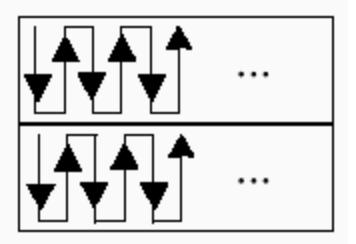
\includegraphics[width=0.5\textwidth]{pic/barre.png} 
    \caption{Légende de cette figure}
    \label{UnNomDeFigure}
\end{figure*}

blablabla....

\section{Structure générale du système}

blablabla....

\begin{figure*}[ht] 
    \centering 
    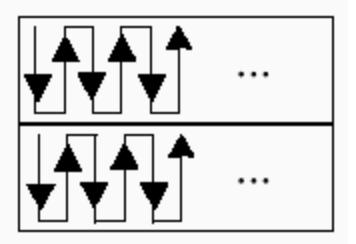
\includegraphics[width=0.9\textwidth]{pic/barre.png} 
    \caption{Légende de cette figure}
    \label{UnAutreNomDeFigure}
\end{figure*}

blablabla....

\chapter{État de l'art / Veille technologique}

Sujet a définir en concertation avec votre encadrant Polytech

\section{Section 1}

PENSEZ à bien insérer TOUTES les références bibliographiques
utilisées dans votre bibliographie.

Voici un exemple de citation: \cite{DBLP:journals/corr/abs-1804-02767}.
Et une autre: \linebreak \cite{DBLP:journals/corr/RedmonDGF15}.

\paragraph{Paragraphe 1}

blablabla

\begin{figure*}[ht] 
    \centering 
    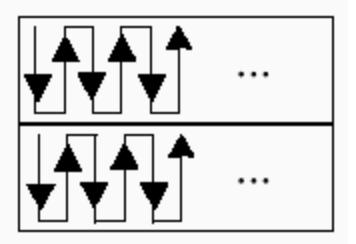
\includegraphics[width=0.5\textwidth]{pic/barre.png} 
    \caption{Fouille de données et visualisation} 
    \label{fdv} 
\end{figure*}

\paragraph{Paragraphe 2}

blablabla

\section{Section 2}

blablabla


\chapter{Analyse et conception}

\section{Analyse}

\subsection{Hypothèses utilisées}
blablabla

\subsection{Spécifications}
Inclure ici un résumé du cahier de spécification qui sera inséré en ANNEXE

\section{Modélisation proposée}

Inclure ici une description du système à développer
pouvant notamment inclure les principaux diagrammes UML non détaillés
et démontrant sa faisabilité durant la phase de mise en œuvre.

Les modes de validation prévus pour les différents éléments à produire
pourront être précisés ici.

\chapter{Mise en oeuvre}

Description de vos productions et de leurs modes de réalisation.

(résumé du cahier de développement inséré en ANNEXE)

blablabla

\section{Outils et librairie utilisés}

blablabla

\section{Éléments d'implémentation, choix techniques}

\begin{lstlisting}[language=C++]
#include <iostream>
using namespace std;

int main () {
    cout << "Hello, world !";
    return 0;
}
\end{lstlisting}

Un exemple de PHP:
\begin{lstlisting}[language=php]
class pdfOrder extends FPDF
{
 function _check($x,$y,$width,$checked) {
   if ($checked)
     $this->rect($x,$y,$width,$width,'F');
   else
     $this->rect($x,$y,$width,$width);
 }
 function LI($sansFrais = false) {
   $LI = 'LI';
   $coord = 'Laboratoire informatique
64, avenue Jean Portalis
37200 Tours
Tél. : 02 47 36 14 42
Fax. : 02 47 36 14 22';
   $this->Image(dirname(__FILE__)  .'/li.jpg',10,2,20);
   $this->SetFont('Times','B',20);
   $this->SetFont('Times','',9);
   $this->setXY(35,3);
   $this->Multicell(80,4,utf8_decode($coord),0,'LT');
 }
\end{lstlisting}

\section{Analyse des résultats, évaluation, qualité}

blablabla


\section{Principales IHM}

\subsection{IHM 1}

Résumé des principaux éléments présent dans le Guide de l'utilisateur
avec d'éventuels compléments d'information sur leur mode de mise en œuvre.


\chapter{Bilan et conclusion}

\section{Bilan du semestre 9}

Liste des taches faites, en cours, à faire
CF Planning S9 et S10 à fournir en annexe

\section{Bilan du semestre 10}

Bilan global $\Rightarrow$ respect du cahier des charges (fait / à faire)

\section{Bilan sur la qualité }
blablabla

\section{Bilan auto-critique}
blablabla

\begin{appendix}
\selectlanguage{french}

\chapter{Planification, gestion de projet}   

\section{Evolution du projet}

Le diagramme de Gantt Initial pour la planification de ce projet 
\img{S10Gantt.png}{Le diagramme de Gantt Final}{width=1.0\textwidth}


Le diagramme de Gantt Final de ce projet est comme Figure A.2.

\img{S10Gantt.png}{Le diagramme de Gantt Final}{width=1.0\textwidth}


\section{Description des tâches}

\paragraph{Tâche 1: Intitulé parlant}

\begin{itemize}
    \item Date de début: 16/09/2019
    \item Date de fin: 03/10/2019
    \item Durée: 17 jours
    \item
        Description: éléments à faire,
        liste des entrées (pré-requis)
        et sorties (livrables)s de la tache.
\end{itemize}

\paragraph{Tâche 2: Intitulé parlant}

\begin{itemize}
    \item Date de début: 16/09/2019
    \item Date de fin: 03/10/2019
    \item Durée: 17 jours
    \item
        Description: éléments à faire,
        liste des entrées (pré-requis)
        et sorties (livrables)s de la tache.
\end{itemize}


\chapter{Description des interfaces}

\section{Interfaces matérielles/logicielles}

blablabla

\section{Interfaces homme/machine}

blablabla

\chapter{Cahier de Spécifications}

\section{spécifications Fonctionnelles}

\subsection{Fonctionnalités à développer}


%~ \setcounter{secnumdepth}{2}
%~ \renewcommand\thesection{\arabic{section}} 

\subsection{ Définition de la fonction 1 : intitulé parlant}

\paragraph{Description de la fonction 1 :}
 
\begin{description}
    \item[Élément 1] ~ \\
        Entrée : ???? \\
        Sortie : ???? \\
        Préconditions : ???? \\
        Postconditions : ????
    \item[Élément 2] ~ \\
        Entrée : ???? \\
        Sortie : ???? \\
        Préconditions : ???? \\
        Postconditions : ????
\end{description}

\subsection{Définition de la fonction 2 :intitulé parlant}

\paragraph{Présentation de la fonction 2:}

\begin{itemize}
    \item Nom de la fonction : Visualisation des statistiques
    \item blablabla
    \item Primordiale
\end{itemize}

\paragraph{Description de la fonction 2 :}

blablabla


\section{Spécifications non fonctionnelles}

\subsection{Contraintes de développement et conception}

blablabla

\subsection{Contraintes de fonctionnement et d’exploitation}

\subsubsection{Performances}
blablabla

\subsubsection{Capacités}
blablabla

\subsubsection{Contrôlabilité}
blablabla

\subsubsection{Sécurité}
blablabla


\chapter{Cahier du développeur}

\section{Introduction}

blablabla

\section{Diagrammes architecturaux et UML}

blablabla

\section{Descriptions détaillées de données exploitées}

blablabla

\section{Descriptions détaillées des classes, modules, réalisations}

blablabla


\chapter{Document d’installation}

Ce document regroupe toutes les informations nécessaires
pour l’installation du projet sur les machines,
ainsi que pour sa mise en production.

\chapter{Document d’utilisation}

blablabla

\chapter{Cahier de test}

Les tests  visent à garantir l'exactitude,
l'intégrité, la sécurité et les performances du logiciel. 

\section{Tests unitaires}

blablabla

\begin{table}[]
\definecolor{C}{HTML}{305496}
\begin{tabular}{|l|l|}\hline
\color{C} IDENTIFICATION OF COMPONENT \\\hline
Afficher toutes les missions de l'utilisateur identifié  \\\hline
\color{C} DESCRIPTION OF THE TEST (granularity, scenario, values, actions) \\\hline
Action :blablabla.\\ blablabla. \\\hline
\color{C} EXPECTED RESULTS \\\hline
Cas 1: blblablaa.\\ Cas 2: blablabla. \\\hline
\color{C} OBTAINED RESULTS \\\hline
blablabla \\\hline
\end{tabular}
\end{table}                                                                             

\section{Tests d'intégration}

blablabla

\end{appendix}

\end{document}


